\documentclass{article}

\usepackage{ctex}
\usepackage{listings}
\usepackage[framed,numbered,autolinebreaks,useliterate]{mcode}
\usepackage{geometry}
\usepackage{multirow}
\usepackage{graphicx}
\usepackage{amsmath}
\usepackage{float}
\geometry{a4paper, scale=0.8}

\title{数学实验实验报告}
\author{ZhaohengLi 2017050025\\cainetatum@foxmail.com\\15801206130}

\begin{document}
\maketitle
\section{实验目的}
\begin{itemize}
	\item{掌握参数估计和假设检验的基本原理和算法;}
	\item{练习使用 MATLAB 解决实际问题。}
\end{itemize}


\section{CH12-T5 接受货物}

\subsection{模型建立}

这是0-1分布的典型案例,记$X=0$表示不合格的货物,$X=1$表示合格的货物。假设货物的真正合格率为$p$,则$X$的均值为$\mu=p$,方差为$\sigma^2=p(1-p)$。根据中心极限定理,样本容量充分大的时候,样本的均值$\overline x$满足$z=\frac{\overline x-\mu}{\sigma / \sqrt n}$近似服从$N(0,1)$,由此对合格品率做如下的假设检验:

$$H_0:p\geq p_0,\quad H_1:p<p_0$$

在这里$p_0$为已知量,为0.9,在这里使用z检验法。


\subsection{算法设计与实现}

可以知道接受域为:

$$z=\frac{\overline x-\mu}{\sigma / \sqrt n}\geq u_\alpha$$

即:

$$\overline x=\sqrt{p_0(1-p_0)/n}*u_\sigma+p_0$$

代码如下:

\begin{lstlisting}
norminv(0.05,0,1)*sqrt(0.9*0.1/50)+0.9
ans = 0.8302

p = fzero(inline('sqrt(p*(1-p)/50)*(-1.6449)+p-0.86'),0.9)
p = 0.9223

n = 152.1868

u = fzero(inline('sqrt(0.9*0.1/50)*u+0.9-0.86'),5)
u = -0.9428

normcdf(u,0,1)
ans = 0.1729

\end{lstlisting}

\subsection{计算结果与分析}

整理计算结果可以得到如下:

$$\overline x = 43/50 = 0.86 > 0.8302$$

这说明样本均值落在接受域内,因此乙应该接受货物。

是否接受货物主要和$p_0,n,\alpha$三个因素相关:

(1)如果甲方承诺的合格率$p_0$高于0.9223,那么这批货物就不应该接受。

(2)如果样本容量加大,提高到153件及以上,那么这批货物不应该被接受。

(3)当双方商定的显著性水平由0.05调高到0.1729,即置信概率由0.95降至0.8271时,不应该接受这批货物。



\section{CH12-T6 身高变化}

\subsection{算法设计与实现}

在第一问中,对于抽取的所有样本数据,可以采用 MATLAB 的 histfit函数进行绘图。该函数既能画出样本分布的直方图,又能够计算估计得到的正态分布曲线。对于正态性的检验,我们设 $H_0$ 代表整体服从正态分布,由于样本数量较大(为 100),所以选用 Jarque-Bera 检验,对应于 MATLAB 中的 jbtest函数。


在第二问中,需要进行参数估计,由于总体的均值 $\mu$ 和方差 $\sigma$ 均为未知量,在进行参数估计 的时候从原理上来讲需要使用样本的方差和均值来计算相应的参数及区间估计。我们可以使 用 MATLAB 的 normfit函数来对正态分布的参数和区间进行估计。


对于第三问,题目中强调 10 年前的数据是普查结果,即为总体的均值,而总体的标准 差未知。对于身高和体重,我们均可以设:$H_0$:均值没有明显变化($\mu = \mu_0$);备选假设$H_1$:均值有明显变化($\mu \neq \mu_0$)。采用 t 检验即可,对应于 MATLAB 中的 ttest函数。


MATLAB代码如下:

\begin{lstlisting}
%% Variables
...

%% Plot
figure;
histfit(height);
xlabel(’Height’);
figure;
histfit(weight);
xlabel(’Weight’);

%% Cal
[mu, sigma, muci, sigmaci] = normfit(height, 0.05) [mu, sigma, muci, sigmaci] = normfit(weight, 0.05)

%% Ttest
h_height = ttest(height, 167.5) h_weight = ttest(weight, 60.2)

\end{lstlisting}



\subsection{计算结果和分析}

对于第一问,学生身高和体重分布的图形描述如下图所示。从图中能够看出,直方图和红 色拟合的正态分布曲线非常接近,从直观上来看分布的确满足“中间高、两段逐渐降低”的 正态分布特点。

并且进一步对身高和体重分别运行jbtest(默认参数)的结果都得到了0,因此假设得到接受,因此身高和体重两个总体均符合正态分布。

\begin{figure}[H]
    \centering
    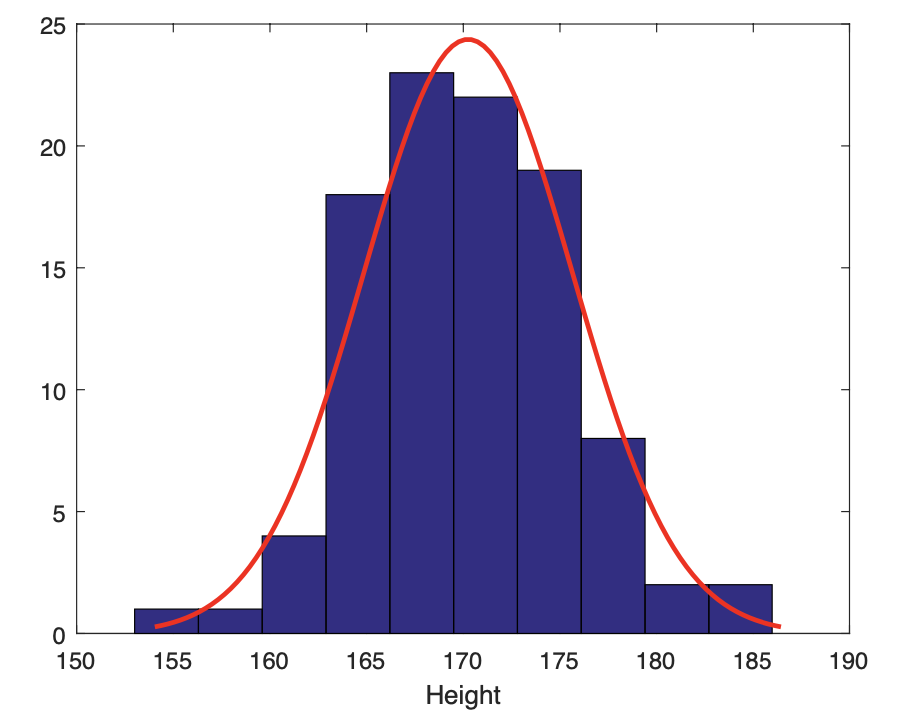
\includegraphics[width=0.4\textwidth]{pic1.png}
    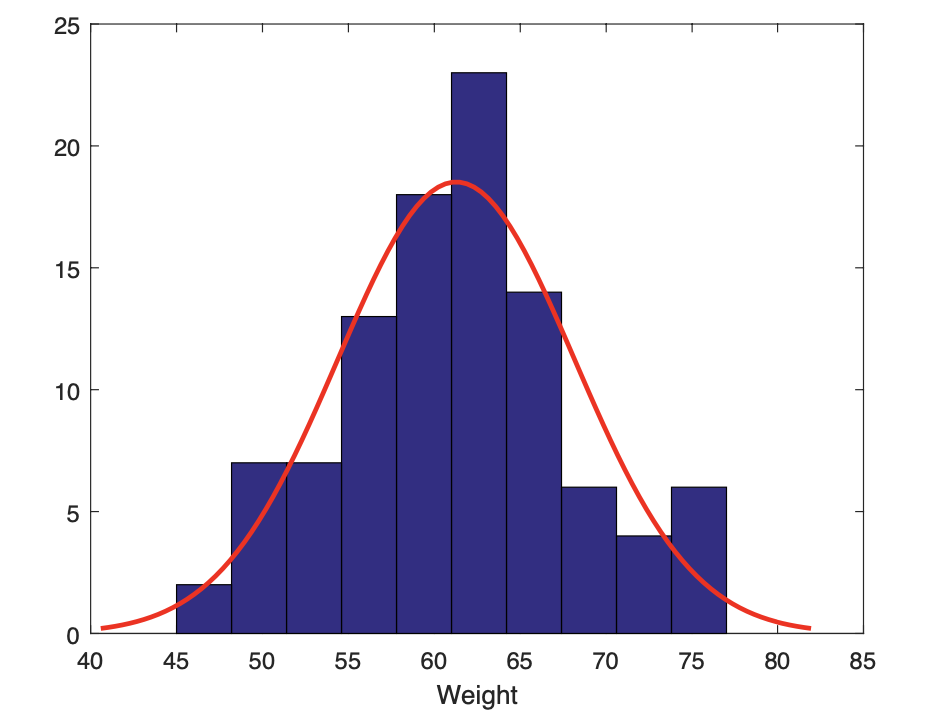
\includegraphics[width=0.4\textwidth]{pic2.png}
\end{figure}

对于第二问,尝试取显著性水平 α 为不同的值进行观察,得出的结果如下表所示。

从表中可以看出,随着显著性水平的减小,参数的区间估计范围也越大,与理论的计算 相符合。

\begin{figure}[H]
    \centering
    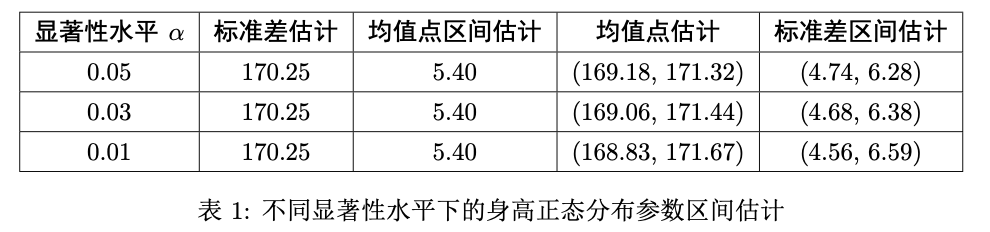
\includegraphics[width=0.8\textwidth]{pic3.png}
    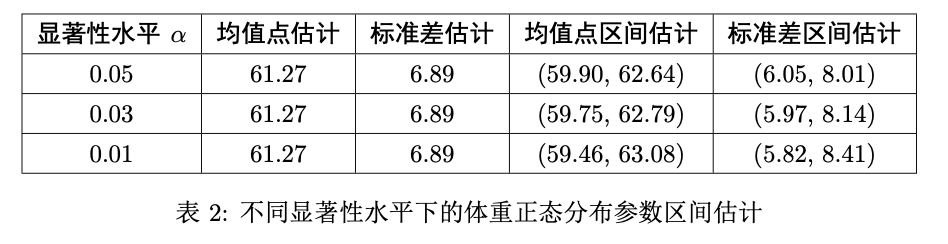
\includegraphics[width=0.8\textwidth]{pic4.png}
\end{figure}


对于第三问,该问选择的显著性水平依然为默认值 α = 0.05,身高和体重进行计算后程序输出分别为1和0,说明学生的身高较 10 年前有了明显的变化,而体重没有明显变化。


\section{CH12-T7 胃溃疡}

\subsection{模型建立}
假设总体患胃溃疡病人的溶菌酶含量和总体正常人的溶菌酶含量均服从正态分布。设总体患胃溃疡病人的溶菌酶含量的均值、方差分别为$\mu_1,\sigma_1$,而正常人的溶菌酶含量的均值、方差分别为$\mu_2,\sigma_2$。

设$\sigma_1^2=\sigma_2^2$且未知,假设检验为:

$$H_0:\mu_1=\mu_2,H_1:\mu_1\neq\mu_2$$

取显著水平为$\alpha = 0.05$


\subsection{算法设计与实现}

代码如下:

\begin{lstlisting}
x1 = [0.2,10.4,...,45.0];
x2 = [0.2,5.4,...,33.0];

[h sig ci] = ttest2(x1,x2,0.05)

m1 = mean(x1)
m2 = mean(x2)
\end{lstlisting}

\subsection{计算结果与分析}
对于第一小问,输出结果为:
\begin{lstlisting}
h = 1
sig = 0.0251
ci = 0.9886 14.3114
m1 = 15.3333
m2 = 7.6833
\end{lstlisting}

可以看出$h=1$应该拒绝$H_0$,即正常人和病人的溶菌酶含量有显著的差别。从其平均值可以看出病人的溶菌酶含量明显高于正常人。


对于第二小问,输出结果为:
\begin{lstlisting}
h = 0
sig = 0.1558
ci = -1.5035 9.1528
m1 = 11.5080
m2 = 7.6833
\end{lstlisting}

从结果上看,应该接受$H_0$。即认为病人的溶菌酶含量和正常人没有显著的区别。

从上述两个结果中可以看出,仅仅删除了5个数据就直接导致了结果的不同。一方面我们可以看到第二次计算得到的均值差别仍然是很大的。但从置信区间和sig可以看出第二次计算结果$H_0$还是非常稳定的。这说明只从均值来判断是不准确的。而且同时说明了原始数据的正确性是十分重要的。有时候需要严谨地去除一些明显不合理的数据点,这样才能够得到更加准确的结果。

\section{实验总结}

通过这次的实验,我学会了使用 MATLAB 求解概率模型参数估计和假设检验问题的一 般方法,并对概率论与数理统计的知识有了更深的理解。希望在之后的课堂上老师能够当堂 进行相关的技巧演示并给出题目的分步解答。

\end{document}